\documentclass[conference]{IEEEtran}
% Shared look for the Rapport papers: packages and TikZ styles for the diagrams.
\usepackage[T1]{fontenc}
\usepackage{amsmath,amssymb}
\usepackage{graphicx}
\usepackage{booktabs}
\usepackage{tabularx}
\usepackage{array}
\usepackage{tikz}
\usetikzlibrary{arrows.meta,positioning,fit,backgrounds,calc,shapes.geometric,shapes.misc}
\usepackage{url}
\usepackage[hidelinks]{hyperref}
\graphicspath{{../figures/}}
\tikzset{
  >={Stealth[length=1.8mm]},
  box/.style={draw, rounded corners=2pt, align=center, font=\scriptsize, minimum height=7mm, inner sep=2pt, fill=#1},
  box/.default=cyan!8,
  code/.style={box=cyan!8},
  llm/.style={box=orange!12},
  io/.style={box=gray!10},
  unity/.style={box=green!10},
  bad/.style={box=red!8},
  good/.style={box=green!12},
  decision/.style={draw, diamond, aspect=2.2, align=center, font=\scriptsize, inner sep=1pt, fill=yellow!12},
  state/.style={draw, circle, align=center, font=\scriptsize, minimum size=12mm, fill=#1},
  state/.default=cyan!8,
  lab/.style={font=\tiny, align=center},
}
\newcolumntype{Y}{>{\raggedright\arraybackslash}X}


\begin{document}

\title{An Integrated, On-Device Architecture for Patient-Specific Embodied Psychiatric Simulation}

\author{\IEEEauthorblockN{Faaz Khan Mohammad}
\IEEEauthorblockA{Rapport project\\
Email: faazkhn1000@gmail.com}}

\maketitle

\begin{abstract}
A simulated psychiatric patient that students can talk to out loud has to do many things at once: hear when the student has finished
speaking, understand the words, decide how the patient feels and what they will say, speak with a fitting tone of voice, and move like a real
person, all within the pause a real patient would leave. For privacy it should do this without sending a student's voice anywhere. This
paper describes how Rapport does all of this on one laptop. The design rests on three ideas. First, \emph{the patient is data}: each case is a
file that lists the patient's memories, mental state, the correct answers and the details that may vary, so a new patient needs no new code.
Second, \emph{code decides and a local language model speaks}: one model call per turn, after code has chosen the patient's mood and allowed
behaviours. Third, \emph{the body reads the same decision as the voice}: the patient's posture, gaze and face follow the emotion code decided.
On an Apple M5 Pro laptop the patient starts speaking a median 1.54\,s after the doctor stops with the earlier patient model, and 1.82\,s with
the new decision layer. A comparison of three local language models kept Gemma 4 E4B as the fastest of the three. A rendering pass moved the
camera to conversation distance, turned the patient to face the doctor, and brought face brightness of all four patient bodies into the
target range (from 0.29--0.44 to 0.49--0.54). We describe each part, show where the time goes, and list the failures we found and fixed.
\end{abstract}

\begin{IEEEkeywords}
virtual patients, embodied conversational agents, speech interfaces, on-device language models, medical simulation, system architecture
\end{IEEEkeywords}

\section{Introduction}
Much of what a psychiatrist notices is not in the words: how slowly someone speaks, how long they pause before answering, whether they look
away, how they sit. Text chat cannot carry these signs. Virtual patients with bodies and voices have been designed for psychiatric interview
practice for years \cite{dupuy2020guidelines}. Recent systems let a language model choose what a 3D patient does \cite{voigt2025llmpowered}
or hold difficult conversations about serious illness \cite{haut2025ai}, and a randomised trial found that patient simulation with
structured feedback improved students' clinical decisions \cite{brugge2024llm}. Most psychiatric language-model patients, however, are still
text chats \cite{wang2024patient,lee2025psyche,sabour2026patientact}.

Building a spoken, embodied psychiatric patient means meeting five requirements at the same time:
\begin{enumerate}
\item \textbf{Speed.} The patient should start speaking within about two seconds; longer feels broken.
\item \textbf{Privacy.} A student's voice and words should not leave the device.
\item \textbf{Patient-specific truth.} Each case is a different person with fixed clinical facts that must never change, even when other
details vary.
\item \textbf{Safety.} Locked memories must stay private, and suicide risk must be handled exactly as the case says.
\item \textbf{One person.} Voice, words and body must agree with each other and stay consistent for the whole interview.
\end{enumerate}
This paper shows how one architecture meets them on a single laptop. A companion paper describes the patient's decision model and its
validation in detail; another describes how memories are recalled from the doctor's words.

\section{Architecture Overview}

\begin{figure*}[t]
\centering
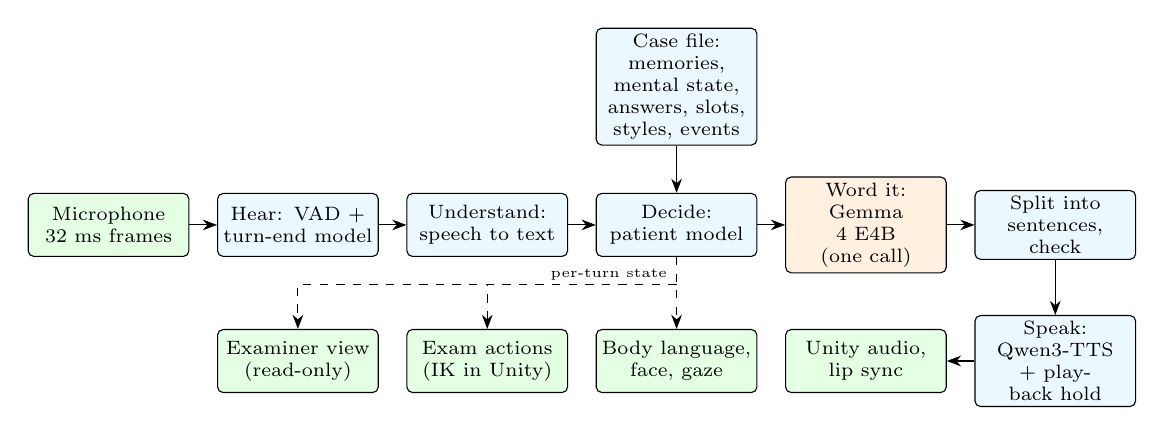
\begin{tikzpicture}[node distance=3mm and 3.5mm]
\tikzset{b/.style={box=#1, text width=19mm, minimum height=8mm}}
\node[b=green!10] (mic) {Microphone\\32 ms frames};
\node[b=cyan!8, right=of mic] (vad) {Hear: VAD +\\turn-end model};
\node[b=cyan!8, right=of vad] (stt) {Understand:\\speech to text};
\node[b=cyan!8, right=of stt] (mind) {Decide:\\patient model};
\node[b=orange!12, right=of mind] (llm) {Word it: Gemma\\4 E4B (one call)};
\node[b=cyan!8, right=of llm] (split) {Split into\\sentences, check};
\node[b=cyan!8, below=7mm of split] (tts) {Speak: Qwen3-TTS\\+ playback hold};
\node[b=green!10, left=of tts] (play) {Unity audio,\\lip sync};
\node[b=green!10, left=of play] (body) {Body language,\\face, gaze};
\node[b=green!10, left=of body] (exam) {Exam actions\\(IK in Unity)};
\node[b=green!10, left=of exam] (twin) {Examiner view\\(read-only)};
\node[b=cyan!8, above=6mm of mind] (case) {Case file: memories, mental state,\\answers, slots, styles, events};
\draw[->] (mic) -- (vad); \draw[->] (vad) -- (stt); \draw[->] (stt) -- (mind); \draw[->] (mind) -- (llm); \draw[->] (llm) -- (split);
\draw[->] (split) -- (tts); \draw[->] (tts) -- (play); \draw[->] (case) -- (mind);
\draw[->, dashed] (mind.south) -- ++(0,-3.5mm) coordinate (b0) -| (body.north);
\draw[->, dashed] (b0) -| (exam.north);
\draw[->, dashed] (b0) -| (twin.north);
\node[lab, anchor=south east, fill=white, inner sep=0.5pt] at ($(mind.south)+(-1mm,-3.2mm)$) {per-turn state};
\end{tikzpicture}
\caption{Rapport's turn loop on one laptop. Blue: the Python patient service; orange: the language model; green: the Unity client and the
examiner's browser. Solid arrows: the path from the doctor's last word to the patient's first sound. Dashed: the patient's state sent to the
body, the exam actions and the examiner view after each turn. Only the read-only examiner view can be opened from another device.}
\label{fig:arch}
\end{figure*}

Three programs run on one Apple M5 Pro laptop with 24\,GB of memory (Fig.~\ref{fig:arch}):
\begin{itemize}
\item a \textbf{Unity~6 client}: the 3D consulting room, the patient's body, the screens the student uses, microphone capture and lip sync;
\item a \textbf{Python patient service}: listening, speech recognition, the patient model, the exam router and speech synthesis;
\item \textbf{llama.cpp} \cite{llamacpp} serving Gemma 4 E4B, a 4-billion-parameter language model, compressed to 4 bits so it fits beside
everything else, with a grammar that forces it to reply in valid JSON.
\end{itemize}
The client and the service talk over one WebSocket per session. No audio or text leaves the laptop.

\section{One Spoken Turn, Step by Step}
Here is what happens between the moment the doctor stops talking and the moment the patient starts. Fig.~\ref{fig:timeline} shows how long
each step takes.

\textbf{1. Hearing the end of the turn.} The microphone sends 32\,ms chunks of sound. A voice-activity detector notices silence and proposes
that the doctor has finished. A small turn-end model then checks the last few seconds of speech and confirms whether the sentence sounded
complete, so the patient does not jump in when the doctor only paused for breath. This takes about 280\,ms.

\textbf{2. Understanding the words.} Speech recognition (Parakeet) starts \emph{speculatively} as soon as the first pause appears, before the
turn is confirmed. If the doctor keeps talking, that work is thrown away; if not, the transcript is usually ready when the turn ends, so the
patient waits only 70--140\,ms for it.

\textbf{3. Deciding.} The patient model runs in code: it reads what the doctor did, adjusts trust, finds the memories the question touches,
applies the trust locks and chooses a short list of allowed behaviours. This takes a few milliseconds.

\textbf{4. Wording it.} One call to the language model. The reply comes back as a stream of JSON, and its fields are ordered so that the
behaviour and emotion arrive \emph{before} the words. The first token arrives after about 280--410\,ms.

\textbf{5. Speaking sentence by sentence.} As soon as the first sentence of the reply is complete, it is checked by code and sent to speech
synthesis, while the model is still writing the rest. Speech synthesis returns its first audio after about 300--350\,ms.

\begin{figure*}[t]
\centering
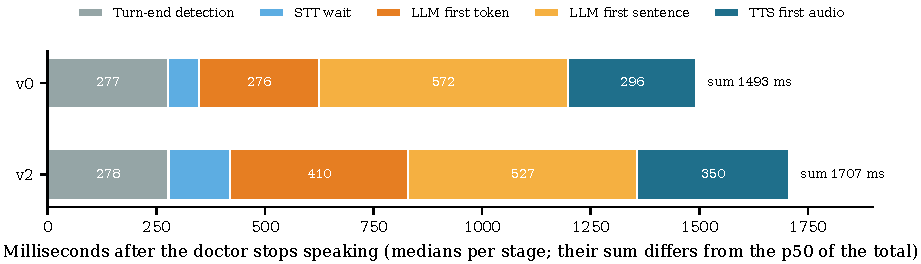
\includegraphics[width=\textwidth]{fig_turn_timeline.pdf}
\caption{Where the time goes in one turn: median time spent in each stage, earlier patient model (v0) and new decision layer (v2). The bars
add up the stage medians, which is close to, but not the same as, the median of the whole turn.}
\label{fig:timeline}
\end{figure*}

\section{The Parts in More Detail}

\subsection{Speaking with feeling}
The voice is Qwen3-TTS 1.7B VoiceDesign, with KittenTTS as a fallback if it fails. This model creates a voice from a written description of the
speaker, and we add the emotion of the moment to that description. Two problems shaped the final design.
\begin{itemize}
\item \textbf{The speaker changed mid-reply.} With this model the description \emph{is} the voice. The first version rebuilt the description for
each sentence as more labels arrived, so sentence two could sound like a different person. Now it is built once per reply, and it carries the
reaction that code decided before the call, scaled by how distressed or agitated the patient is.
\item \textbf{The voice broke up when the computer was busy.} Speech synthesis runs about twice as fast as real time when the computer is free,
but only about real time while the language model is also running. Audio sent from the first chunk then ran out mid-word. The service now holds
each sentence until the audio already buffered is longer than the time it will take to make the rest. On a free computer this costs nothing.
\end{itemize}
The model ignores a speed setting, so fast, pressured speech or slow, depressed speech is created with words in the description (``speaking fast,
words tumbling out'') and a time-stretch that keeps the pitch the same.

\subsection{The body}
Four patient bodies, two of each sex, share one skeleton and one set of face shapes, so every movement works on all of them. After each turn the
patient model sends its state (emotion, reaction, intensity from 0 to 10, behaviour, resistance and the four state values). A body-language
component turns that into movement, blended smoothly and scaled by intensity (Table~\ref{tab:body}, Fig.~\ref{fig:body}). It always gives way to
physical-examination actions and to standing up.

\begin{table}[t]
\caption{How the patient model's emotion becomes body language}
\label{tab:body}
\centering
\scriptsize
\begin{tabularx}{\columnwidth}{@{}lY@{}}
\toprule
Emotion & What the body does\\
\midrule
Angry, hostile & leans in, turns the head away and back, sets the jaw, sharp hand gesture\\
Anxious & fidgets, raises the shoulders, bounces a knee, quick glances\\
Sad & slumps, head and eyes down, slower movements\\
Ashamed & slumps, eyes down, turns slightly aside\\
Happy & small smile; a short laugh at high intensity\\
Confused & tilts the head\\
Suspicious & sits back, slightly side-on\\
Flat & barely moves\\
\midrule
Always (idle life) & blinks about 17 times a minute (1 in 8 a double blink); small eye movements; breathing that quickens with anxiety or
anger; a posture shift every 8--20\,s; eyes wander while ``thinking''; nods while the doctor talks; eye contact that rises with trust and falls
with shame or sadness\\
\bottomrule
\end{tabularx}
\end{table}

\begin{figure*}[t]
\centering
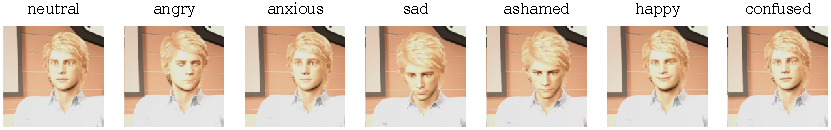
\includegraphics[width=\textwidth]{fig_body_language.pdf}
\caption{Body language driven by the patient model's emotion (one frame each, high intensity, from a scripted sequence on one body).}
\label{fig:body}
\end{figure*}

\subsection{Physical examination}
Requests such as ``hold out your hands'', ``roll up your sleeves'', ``look at this light'' or ``stand up and walk'' are recognised by rules, not by
the language model. On 385 test sentences the rules chose the exact action every time, with no false triggers on 56 sentences that were not
requests (one author wrote both the rules and the test, so this is optimistic). Trust and agitation decide whether the patient complies; below
the case's level, the patient refuses in their own words. Actions play with inverse kinematics: palms turn with the forearm, sleeves roll up with
shapes generated at run time, held hands show the case's tremor, and sweating shows as a sheen on the skin.

\subsection{The examiner view}
A web page shows the patient model's state live: trust, distress, agitation and engagement; the mood over time; memories unlocking as trust
rises; and a one-line reason for each reply written by code (for example ``Mood memory open (trust 39 $\ge$ 20). Touched something locked (needs
trust 55); showed discomfort.''). An examiner can open it on a second laptop on the same network. Nothing else on the service answers other
devices.

\subsection{One brain for typed and spoken turns}

\begin{figure}[t]
\centering
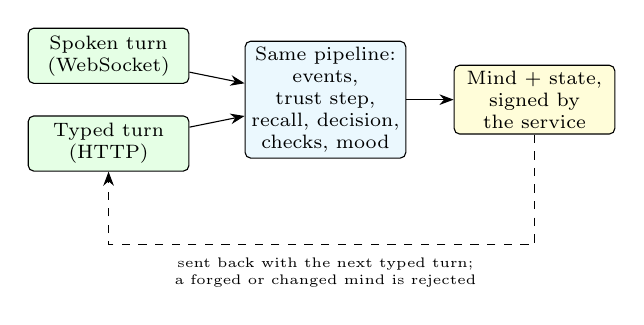
\begin{tikzpicture}[node distance=4mm and 5mm]
\tikzset{b/.style={box=#1, text width=19mm}}
\node[b=green!10] (voice) {Spoken turn\\(WebSocket)};
\node[b=green!10, below=of voice] (typed) {Typed turn\\(HTTP)};
\node[b=cyan!8, anchor=west] (mind) at ($(voice.east)!0.5!(typed.east)+(7mm,0)$) {Same pipeline:\\events, trust step,\\recall, decision,\\checks, mood};
\node[b=yellow!15, right=6mm of mind] (sig) {Mind + state,\\signed by\\the service};
\draw[->] (voice) -- (mind); \draw[->] (typed) -- (mind); \draw[->] (mind) -- (sig);
\draw[->, dashed] (sig.south) |- ++(0,-14mm) -| (typed.south);
\node[lab, text width=48mm, fill=white] at ($(mind.south)+(0,-14.5mm)$) {sent back with the next typed turn;\\a forged or changed mind is rejected};
\end{tikzpicture}
\caption{Typed and spoken turns use the same pipeline. For typed turns the client carries the patient's mind between requests, signed so that
it cannot be forged.}
\label{fig:paths}
\end{figure}

Students can also type. Typed turns go through the same pipeline as spoken ones (Fig.~\ref{fig:paths}). Each typed reply returns the patient's new
state and its \emph{mind}: mood, the memory of the conversation, resistance and which events have happened. The client sends the mind back with
the next request. The service signs it with a secret key and accepts only minds it issued, so a client can neither invent memories nor slip
instructions into the prompt; a changed or oversized mind simply starts fresh. Before this change, typed turns skipped events, the trust step and
the mood update, and an independent review found that the mind was also silently thrown away, so the typed patient forgot everything each turn.

\section{The Patient Is Data}

\begin{figure}[t]
\centering
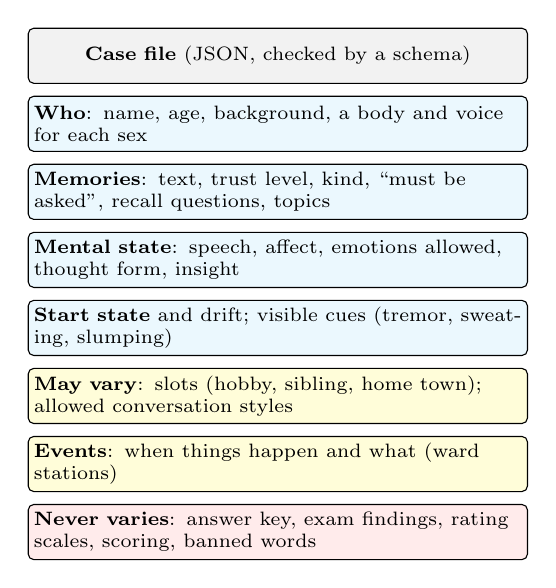
\begin{tikzpicture}[node distance=1.5mm]
\tikzset{b/.style={box=#1, text width=62mm, align=left, font=\scriptsize}}
\node[box=gray!10, text width=62mm] (root) {\textbf{Case file} (JSON, checked by a schema)};
\node[b=cyan!8, below=of root] (id) {\textbf{Who}: name, age, background, a body and voice for each sex};
\node[b=cyan!8, below=of id] (mem) {\textbf{Memories}: text, trust level, kind, ``must be asked'', recall questions, topics};
\node[b=cyan!8, below=of mem] (mse) {\textbf{Mental state}: speech, affect, emotions allowed, thought form, insight};
\node[b=cyan!8, below=of mse] (st) {\textbf{Start state} and drift; visible cues (tremor, sweating, slumping)};
\node[b=yellow!15, below=of st] (var) {\textbf{May vary}: slots (hobby, sibling, home town); allowed conversation styles};
\node[b=yellow!15, below=of var] (ev) {\textbf{Events}: when things happen and what (ward stations)};
\node[b=red!8, below=of ev] (key) {\textbf{Never varies}: answer key, exam findings, rating scales, scoring, banned words};
\end{tikzpicture}
\caption{What a case file holds. Yellow parts may vary with a seed; red parts never change.}
\label{fig:case}
\end{figure}

Every patient is a case file (Fig.~\ref{fig:case}), checked against a schema when it loads. Making a new patient means writing a new file, not new
code. There are four draft stations today:
\begin{itemize}
\item \textbf{Moderate depression}: a 24-year-old software tester, two months of low mood, early waking, and a passive wish not to wake up.
\item \textbf{``I want to go home''}: the same patient a week later on a ward, asking to leave, under India's Mental Healthcare Act \cite{mhca2017}.
\item \textbf{``I'm not taking those tablets''}: a young patient refusing medicine, guarded and suspicious.
\item \textbf{Alcohol dependence with early withdrawal}: a sales manager whose hands shake in the morning, with a past withdrawal fit
\cite{nice2010cg100}.
\end{itemize}

\subsection{Seeded patients: different people, same answers}
A \emph{seed} (any number) picks one option for each ``slot'' and one conversation style. The same seed always gives the same patient. In the
depression case the slots are a hobby (Carnatic singing, badminton, guitar or drawing), a younger brother's name (Rohan, Karthik or Varun) and a home
town (four options). The answer key never changes: across 40 seeds, the correct answers, scales, exam findings, every trust level and all risk
memories stayed identical to the authored case. Table~\ref{tab:styles} shows the six conversation styles \cite{wang2024patient}. Each style has a
part the model sees (a label, a description and example lines) and a part code enforces (numbers that change how trust and agitation move, and a
limit on how many words the patient says).

\begin{table}[t]
\caption{Conversation styles: what code enforces (draft numbers)}
\label{tab:styles}
\centering
\scriptsize
\begin{tabular}{@{}lccccc@{}}
\toprule
Style & Start change & Trust up/down & Agit. & Words & Softens\\
\midrule
Plain & none & 1.0 / 1.0 & 1.0 & 120 & --\\
Reserved & T$-$5, E$-$10 & 0.8 / 1.2 & 1.0 & 20 & T 45\\
Eager to please & T+5 & 1.2 / 0.8 & 0.8 & 35 & --\\
Upset & T$-$10, A+15 & 0.7 / 1.2 & 1.3 & 35 & T 40\\
Talkative & E+10 & 1.0 / 1.0 & 1.0 & 70 & --\\
Tangential & none & 1.0 / 1.0 & 1.0 & 70 & --\\
\bottomrule
\end{tabular}
\\[1mm]\raggedright\scriptsize T trust, E engagement, A agitation. ``Softens'': trust at which the style relaxes.
\end{table}

\subsection{Ward events}
On ward stations, things happen during the interview. \emph{Code} decides when; the language model only acts it out, from a stage direction it is
told never to read aloud (and any sentence that copies it is dropped). Fig.~\ref{fig:events} shows the events of the ``I want to go home''
station. Against a coercive typed doctor (``You can't go home'', ``calm down''), the patient's trust fell from 25 to 0 and agitation rose from 45 to
92, and the patient stood up; against a doctor who explored reasons, explained rights honestly and offered choices, trust rose to 70 and agitation
fell to 25.

\begin{figure}[t]
\centering
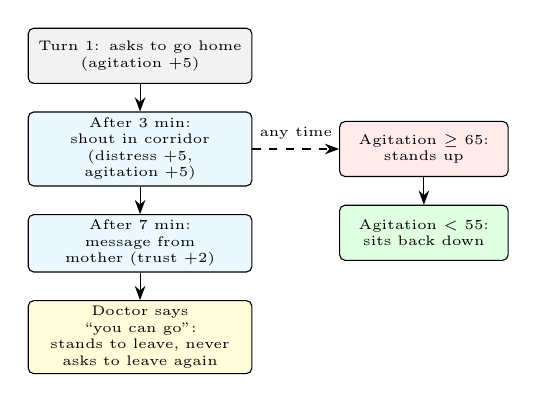
\begin{tikzpicture}[node distance=3.5mm]
\tikzset{b/.style={box=#1, text width=27mm, font=\tiny}}
\node[b=gray!10] (start) {Turn 1: asks to go home\\(agitation +5)};
\node[b=cyan!8, below=of start] (shout) {After 3 min: shout in corridor\\(distress +5, agitation +5)};
\node[b=cyan!8, below=of shout] (mum) {After 7 min: message from\\mother (trust +2)};
\node[b=yellow!15, below=of mum] (go) {Doctor says ``you can go'':\\stands to leave, never\\asks to leave again};
\node[b=red!8, right=11mm of shout, text width=20mm] (stand) {Agitation $\ge$ 65:\\stands up};
\node[b=green!12, below=of stand, text width=20mm] (sit) {Agitation $<$ 55:\\sits back down};
\draw[->] (start) -- (shout); \draw[->] (shout) -- (mum); \draw[->] (mum) -- (go);
\draw[->, dashed] (shout) -- node[lab, above]{any time} (stand); \draw[->] (stand) -- (sit);
\end{tikzpicture}
\caption{Events in the ``I want to go home'' ward station. Each fires at most once, when its condition first holds.}
\label{fig:events}
\end{figure}

A tester found a loop: after ``You're free to go home'', the patient denied it and asked to go home again, over and over. Two fixes closed it.
Permission to leave is now recognised in 24 everyday phrasings (``You can head home'', ``Off you go'', ``Go home if you want'', ``I'm discharging
you''), while 16 refusals, conditions and questions (``You can't go home'', ``If you feel better you can go'') are not. Once permission is given,
any sentence asking to leave again is dropped before it is spoken. Replayed on the real model, the patient asked what happens next and worried
about their job, and never asked to leave again.

\section{Results}

\subsection{Speed}
Table~\ref{tab:lat} and Fig.~\ref{fig:lat} show the time from the doctor's last sound to the patient's first sound, taken from the service's own
timing log, with nothing else using the graphics processor. The new decision layer added 279\,ms at the median. Most of it is in the first token
(+134\,ms) and the speech-recognition wait (+70\,ms). We also tried two other local models as the patient. Both were slower (medians 2.19\,s and
2.88\,s). On one test run the judge flagged 53 and 62 replies with unsupported claims for them, against 1--8 per run for Gemma; the judges differed
(no model judged itself), so this is only an indication. Gemma 4 E4B stays.

\begin{table}[t]
\caption{Time per stage, median milliseconds}
\label{tab:lat}
\centering
\footnotesize
\begin{tabular}{@{}lrrrr@{}}
\toprule
Stage & v0 & v2 & Q3.5-4B & Q3.5-9B\\
\midrule
Turn-end detection & 277 & 278 & 278 & 279\\
Speech-to-text wait & 72 & 142 & 156 & 180\\
Model first token & 276 & 410 & 424 & 599\\
Model first sentence & 848 & 937 & 950 & 1385\\
Speech first audio & 296 & 350 & 758 & 983\\
\midrule
\textbf{Patient audio ready, median} & \textbf{1540} & \textbf{1819} & \textbf{2186} & \textbf{2882}\\
90th percentile & 2560 & 2962 & 2824 & 4126\\
Turns measured & 80 & 37 & 22 & 22\\
\bottomrule
\end{tabular}
\end{table}

\begin{figure}[t]
\centering
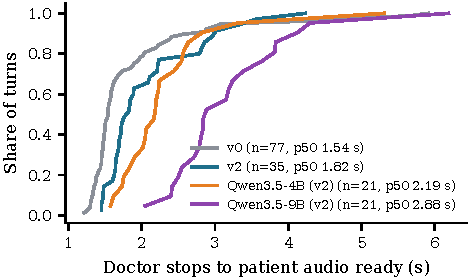
\includegraphics[width=\columnwidth]{fig_latency.pdf}
\caption{How long patients took to start speaking, as a cumulative share of turns.}
\label{fig:lat}
\end{figure}

\subsection{How the patient looks}
Before the rendering pass, the doctor's camera showed a wide shot with the face only about 67 pixels wide, the faces were darker than the room,
and every patient sat turned away (their seat faced about 156 degrees from the doctor). Now the seat faces the doctor at 110 degrees, the camera
frames the patient at conversation distance (face about 142 pixels wide), and a soft light that only shines on the patient brightens the face
without brightening the room. Face brightness moved into the target range for all four bodies (Fig.~\ref{fig:lum}, Fig.~\ref{fig:stills},
Fig.~\ref{fig:bodies}) with no washed-out pixels. The closer view also revealed that two imported bodies were drawn without hair and eyes from some
angles, because their size boxes were wrong; they are now computed from the skeleton. Rendering one frame at 1920$\times$1080 took 6.4--8.1\,ms in
the editor. The 60-frames-per-second check in the finished app, during a live conversation, has not been run yet.

\begin{figure}[t]
\centering
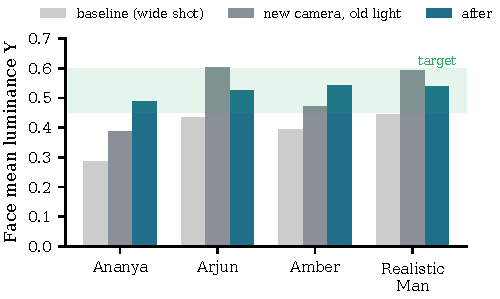
\includegraphics[width=\columnwidth]{fig_luminance.pdf}
\caption{Face brightness of the four bodies; green band: target.}
\label{fig:lum}
\end{figure}

\begin{figure*}[t]
\centering
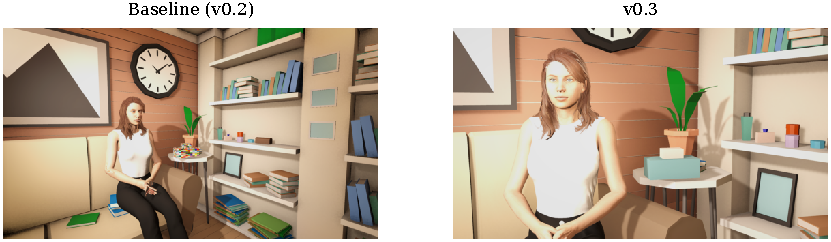
\includegraphics[width=\textwidth]{fig_stills.pdf}
\caption{The doctor's view before and after the rendering pass (same body).}
\label{fig:stills}
\end{figure*}

\begin{figure}[t]
\centering
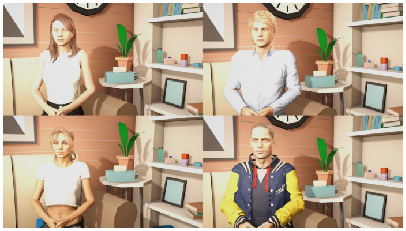
\includegraphics[width=\columnwidth]{fig_bodies.pdf}
\caption{All four bodies from the doctor's seat after the rendering pass.}
\label{fig:bodies}
\end{figure}

\subsection{Failures we found, and what they teach}
\begin{itemize}
\item \textbf{Two programs sharing one model slot mixed up replies.} During one test a replay script and a timing benchmark used the same model
server and the same reserved slot at the same time, and replies went to the wrong program. A live session has only one client, so students were
not affected, but test runs must never share the patient's model server.
\item \textbf{Typed turns forgot everything}, as described above.
\item \textbf{The timing benchmark crashed} when the service decided the doctor had finished before the recorded sentence ended; it now records
this as an ``early turn end'' and carries on.
\item \textbf{The voice changed speaker mid-reply}, because the voice description changed between sentences.
\end{itemize}

\section{Discussion and Limitations}
The main trade-off is between deciding more in code and starting to speak sooner. Each check is cheap, but holding a whole reply back on a risk
turn (so a denial can be replaced) and the longer prompt both cost time. A median of 1.8\,s is close to the thoughtful pause of a low-mood
patient, but misses a 1.2\,s target for brisker cases. Other limits: only one laptop model was measured; lip sync is still weak (the mouth opens
mostly with the jaw); skin, eye and hair shading use the standard pipeline; and no students have used this version yet.

\section{Conclusion}
A spoken, embodied psychiatric patient can run privately on one laptop if the patient is data, code makes the decisions, a local model speaks, and
the body reads the same decision as the voice. Each of these choices made a class of failure visible and fixable.

\section*{Ethics}
No human participants or real patient data were involved. Voices are designed from written descriptions, not copied from real people. All clinical
content is draft until faculty review it.

\bibliographystyle{IEEEtran}
\bibliography{../shared/refs}

\end{document}
